% cat-deep-merge.tex — the deep merge: rec + recurses key by key and bags every other colliding value, a lst whole.
% Rendered with the tikz MCP server (compile_tikz), which wraps this body in a
% standalone document (default preamble: tikz, amsmath, amssymb + common TikZ
% libraries) and writes docs/website/skills/mtron/assets/cat-deep-merge.png.
%
% INK: white on a transparent background — the site's theme is dark (--maincolor
% #000000, panels #191C24). Labels are UNFILLED and set clear of the strokes.
%
% THE FIGURE, IN ONE PICTURE. Two weekend walk reports (the dogs mama, puppy and chelsea) merged, sat + sun. Every framed key
% is in BOTH reports and merges key by key; a leaf records the rule that made it. A lst is an ATOM of the
% merge: two colliding lsts bag whole (a bag of lsts), and only a select's + concatenates them.
%
%                                     sat + sun
%               [mama]                  [puppy]                  [chelsea]
%         [km]      visited=>{[arroyo],[acequia,mesa]}     [km]                [km]
%  ridge=>{12,9}  lake=>5   [arroyo] ⊎ [acequia,mesa]    ridge=>12  lake=>5    lake=>{2}5
%     12 ⊎ 9    Saturday's alone                     Saturday's Sunday's  5 ⊎ 5 = {2}5

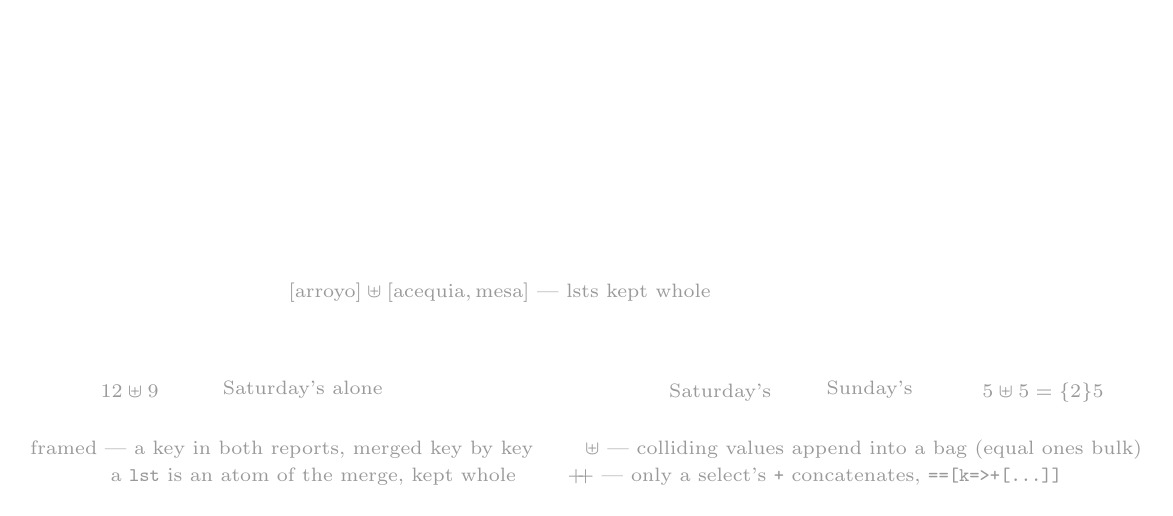
\begin{tikzpicture}[
  k/.style={draw, rounded corners=2pt, thick, minimum height=6.5mm, inner sep=1.2mm, font=\small},
  leaf/.style={font=\small, inner sep=1pt},
  e/.style={thick},
  sub/.style={font=\scriptsize, text=white!60!black, inner sep=1pt},
  color=white
]
% the merged report — every framed key is in both reports, so it merges key by key
\node[k] (root) at (0,0) {$\mathrm{sat} + \mathrm{sun}$};

\node[k] (maya) at (-3.7,-1.3) {\texttt{mama}};
\node[k] (tom)  at ( 2.2,-1.3) {\texttt{puppy}};
\node[k] (ines) at ( 5.4,-1.3) {\texttt{chelsea}};

\node[k]    (mkm)  at (-5.2,-2.6) {\texttt{km}};
\node[leaf] (msum) at (-1.5,-2.6) {\texttt{visited=>\char`\{[arroyo],[acequia,mesa]\char`\}}};
\node[k]    (tkm)  at ( 2.2,-2.6) {\texttt{km}};
\node[k]    (ikm)  at ( 5.4,-2.6) {\texttt{km}};

\node[leaf] (mr) at (-6.2,-3.9) {\texttt{ridge=>\char`\{12,9\char`\}}};
\node[leaf] (ml) at (-4.0,-3.9) {\texttt{lake=>5}};
\node[leaf] (tr) at ( 1.3,-3.9) {\texttt{ridge=>12}};
\node[leaf] (tl) at ( 3.2,-3.9) {\texttt{lake=>5}};
\node[leaf] (il) at ( 5.4,-3.9) {\texttt{lake=>\char`\{2\char`\}5}};

\foreach \a/\b in {root/maya, root/tom, root/ines, maya/mkm, maya/msum, tom/tkm, ines/ikm, mkm/mr, mkm/ml, tkm/tr, tkm/tl, ikm/il}
  \draw[e] (\a) -- (\b);

% the rule each leaf records
\node[sub, anchor=north] at ([yshift=-2pt]mr.south)   {$12 \uplus 9$};
\node[sub, anchor=north] at ([yshift=-2pt]ml.south)   {Saturday's alone};
\node[sub, anchor=north] at ([yshift=-2pt]msum.south) {$[\mathrm{arroyo}] \uplus [\mathrm{acequia}, \mathrm{mesa}]$ — lsts kept whole};
\node[sub, anchor=north] at ([yshift=-2pt]tr.south)   {Saturday's};
\node[sub, anchor=north] at ([yshift=-2pt]tl.south)   {Sunday's};
\node[sub, anchor=north] at ([yshift=-2pt]il.south)   {$5 \uplus 5 = \{2\}5$};

% the legend
\node[sub, anchor=north, align=center] at (-0.4,-4.85)
  {framed — a key in both reports, merged key by key \qquad $\uplus$ — colliding values append into a bag (equal ones bulk)\\[2pt]
   a \texttt{lst} is an atom of the merge, kept whole \qquad $\mathbin{+\!\!+}$ — only a select's \texttt{+} concatenates, \texttt{==[k=>+[\ldots]]}};
\end{tikzpicture}
